\documentclass[conference]{IEEEtran}
% \documentclass[conference]{../sty/IEEEtran}

% *** CITATION PACKAGES ***
%\usepackage{cite}


% *** GRAPHICS RELATED PACKAGES ***
\usepackage[pdftex]{graphicx}
% \graphicspath{{../pdf/}{../jpeg/}}
% \DeclareGraphicsExtensions{.pdf,.jpeg,.png}

% *** MATH PACKAGES ***
\usepackage[cmex10]{amsmath}
%\interdisplaylinepenalty=2500

% *** SPECIALIZED LIST PACKAGES ***
%\usepackage{algorithmic}

% *** ALIGNMENT PACKAGES ***
\usepackage{array}
%\usepackage{mdwmath}
%\usepackage{mdwtab}

%\usepackage{eqparbox}

% *** SUBFIGURE PACKAGES ***
\usepackage[caption=false,font=footnotesize]{subfig}

% *** FLOAT PACKAGES ***
%\usepackage{fixltx2e}
%\usepackage{stfloats}
%\fnbelowfloat

% *** PDF, URL AND HYPERLINK PACKAGES ***
%\usepackage{url}
% \url{my_url_here}.

% correct bad hyphenation here
%\hyphenation{op-tical net-works semi-conduc-tor}


%================================================================================================
\begin{document}

\title{Detection of sentence modality on\\French automatic speech-to-text transcriptions}

\author{\IEEEauthorblockN{Luiza Orosanu, Denis Jouvet}
\IEEEauthorblockA{Speech Group, LORIA\\
Inria, Villers-l\`{e}s-Nancy, F-54600, France \\
Universit\'{e} de Lorraine, LORIA, UMR 7503, Villers-l\`{e}s-Nancy, F-54600, France \\
CNRS, LORIA, UMR 7503, Villers-l\`{e}s-Nancy, F-54600, France \\
Email: \{luiza.orosanu, denis.jouvet\}@loria.fr}
}


\maketitle


\begin{abstract}
This article analyzes the detection of sentence modality in French when it is applied on automatic speech-to-text transcriptions. 
Two sentence modalities are evaluated (questions and statements) using prosodic and linguistic information. 
The linguistic features consider the presence of discriminative interrogative patterns and two log-likelihood ratios of the sentence being a question rather than a statement: one based on words and the other one based on part-of-speech tags. 
The prosodic features are based on duration, energy and pitch features estimated over the last prosodic group of the sentence. 
The classifiers based on linguistic features outperform the classifiers based on prosodic features. 
The combination of linguistic and prosodic features gives a slight improvement on automatic speech transcriptions, where the correct classification performance reaches 72\%. 
A detailed analysis shows that small errors in the determination of the segment boundaries are not critical.
\end{abstract}
\begin{IEEEkeywords}
question detection, speech-to-text transcriptions, prosody, likelihood ratio, part-of-speech tags
\end{IEEEkeywords}


%================================================================================================
\section{Introduction}
%================================================================================================

The work presented in this paper is part of the RAPSODIE project, which aims at studying, deepening and enriching the extraction of relevant speech information, in order to support communication with deaf or hard of hearing people. 
The detection of sentence modality (questions versus statements) is a key problem here, the deaf or hard of hearing people must be informed when a question is directed to them, and that they should respond or ask for further clarifications (if needed). 
Therefore, we are interested in finding a solution that performs well on automatic speech-to-text transcriptions (its accuracy depends on the sound quality and on the performance of the speech recognition system).

The automatic detection of questions has been studied in the past decades with different objectives: to model and detect the speech structure \cite{Jurafsky:1997}, to detect the sentence modality (mainly statements versus questions) \cite{Kral:2005, Yuan:2005, Quang:2006, Quang:2007, Khan:2010, Margolis:2011}, to create the summary of documents or meetings \cite{Quang:2006}, to enrich an automatic transcription with punctuation marks \cite{Kolar:2012}, etc.

Most of the studies are only based on correct data (textual and/or audio), without being related to any automatic speech recognition systems.  
A detector of French questions (versus declarative and exclamatory sentences) was designed in \cite{Kral:2005} using only prosodic features (pitch and energy) computed on the last 700 milliseconds of speech.
Prosodic based classifiers were also studied for the Arabic language \cite{Khan:2010}. The energy and the fundamental frequency were the key features in their classifier. 

Another detector of French questions (versus declarative sentences) was designed in \cite{Quang:2006, Quang:2007}. They first started off with only prosodic features and soon realized that using other cues like the lexical information can improve its performance on spontaneous speech.

In \cite{Liscombe:2006} the English question asking behavior was designed in order to improve the intelligent tutoring systems. Their study concluded that the most useful features were prosodic, in particular the pitch slope of the last 200 milliseconds of a turn. 

The studies related to automatic speech recognition systems have to additionally take into account word error rates, poor sound qualities, spontaneous speech, which can highly decrease the classification performance.
In \cite{Jurafsky:1997}, 42 dialog acts were used to model and detect the discourse structure of natural English speech (human-to-human telephone conversations). They used three different types of information (linguistic, prosodic and a statistical discourse grammar) and achieved an accuracy of 65\% on ASR transcripts versus 72\% on reference manual transcripts. Combining recognized words with the discourse grammar was the most useful for this task. 

The detection of questions in English meetings was addressed in \cite{Boakye:2009}. They used lexico-syntactic, turn related and pitch related information and achieved an accuracy of 54\% on ASR transcripts versus 70\% on reference manual transcripts. The lexico-syntactic features were the most useful for this task.
The automatic punctuation (comma, period, question mark) of French and English speech-to-text data was studied in \cite{Kolar:2012}. Their boosting-based model uses linguistic (based on word n-grams) and prosodic information and was tested under real world conditions. 

All of the mentioned classifiers are applied on different languages, on different data, on different conditions, and with different features. Some use data sets that are already manually classified in dialog acts, others extract sentences from their data sets based on the punctuation marks (with or without posterior manual relabeling). Some, based on the general opinion that a question's intonation has a final rising pitch \cite{Cristo:1998}, are interested only in the last part of the speech signal, others on the whole sentence. Some compute various prosodic coefficients (even up to 123 different coefficients), others keep only the most classic values: mean, maximum, minimum, delta, slope, etc. Every analysis is unique and very dependent on the data and on the choice of features. 

In our study several approaches are analyzed: creating a classifier with only prosodic features (extracted from the acoustic signal) or one with only linguistic features (extracted from the word and part-of-speech sequences) or one that combines both linguistic and prosodic features. The classifier evaluations are carried out using linguistic features stemming out from automatic speech-to-text transcriptions (to study the performance under real conditions) and from manual transcriptions (to study the performance in ideal conditions - i.e. when there are no word errors). 

The novelty of our approach consists in combining 3 different types of linguistic features (word-based n-grams, PartOfSpeech-based n-grams and the presence of discriminative interrogative patterns) to detect questions in French automatic speech-to-text transcriptions. The first experiments are conducted on perfect (predefined) sentence boundaries. 
Then we evaluate the performance loss when sentence boundaries are not perfect (by changing those boundaries randomly or relative to silence/noise decoded units).

The paper is organized as follows: section 2 is devoted to the description of the data and tools used in our experiments, section 3 provides a description of the features used for question detection, and section 4 presents and analyzes the results.


%=======================================================================================
\section{Experimental setup}
%=======================================================================================

\subsection{Textual data for training language models}

Textual punctuated data is necessary for modeling the lexical and syntactic characteristics of questions and statements. 

The available textual data corresponds to more than 800 million words from the French Gigaword corpus \cite{Mendonca:2011}. Based on a unique list of 97K words, 89K questions and 16M statements were extracted out of this corpus by filtering the sentences ending with a question mark, respectively with a dot. The lexical data was also annotated with part-of-speech (POS) tags (thus providing the syntactic data).

Based on the lexical (word-based) data we learned two language models, one for questions and one for statements (with a shared lexicon of 97K words). 
These language models have the purpose of representing the main sequences that occur respectively in questions and in statements (like for example in French: ``est-ce que ...", ``qu'est-ce que ...", etc).

Based on the syntactic (POS-based) data we learned two other language models, one for questions and one for statements (with a shared lexicon of 36 POS tags). 
These language models have the purpose of representing the main syntactic sequences that occur respectively in questions and in statements (like for example in French the verb-pronoun inversions: ``regardez vous ...", ``pourrait on ...", ``fallait il ...", etc).

Table \ref{Tab:LMs} describes the resulting 3-gram language models based on questions and statements, when using words-based sentences or POS-based sentences.

\begin{table}[!b]
\renewcommand{\arraystretch}{1.3}
\caption{Number of 3-grams in the language models computed over questions and statements}
\label{Tab:LMs}
\centering
\begin{tabular}{|r|r|r|}
\hline
{\bf Language model}  & word-based  & POS-based 	\\ \hline
questions     & 718K  &  9K  	\\ \hline
statements    &  68M  & 16K   	\\ \hline
\end{tabular}
\end{table}


\subsection{Speech and textual data for question detection}\label{data}

The speech corpora used to train and evaluate the question detection classifiers come from the ESTER2 \cite{Galliano:2009} and ETAPE \cite{Gravier:2012} evaluation campaigns, and the EPAC \cite{ESTEVE:2010} project. 
The ESTER2 and EPAC data are French broadcast news collected from various radio channels (prepared speech and interviews). 
The ETAPE data correspond to debates collected from various radio and TV channels (spontaneous speech). 
These corpora were manually transcribed and punctuated (the segmentation of speech into sentences is therefore already given).

The set of questions and statements were extracted from these corpora by filtering the sentences ending with a question mark and respectively with a dot.
The training sets of ESTER2, EPAC and ETAPE corpora are used to train the question detection classifiers; the development and test sets of the ESTER2 and ETAPE corpora are used to evaluate them.

The speech training data set contains 10K questions and 98K statements. 
However, binary classifiers do not work well when trained on imbalanced data sets: new instances are likely to be classified as the class that has more training samples. %receive the tag of the class with more training samples.
In order to avoid this overfitting problem, we chose to resample the data set by keeping all questions and randomly extracting subsets of statements of the same size (ten different training data sets are considered based on the different random lists of statements). 
In the 'Experiments and results' section we present only the average performance (with the associated standard deviations) over all ten training data sets. 

The evaluation data set is kept intact. 
Table \ref{Tab:usedData} gives more details on the number of questions and statements used in our experiments.  

\begin{table}[!b]
\renewcommand{\arraystretch}{1.3}
\caption{Description of the data used in our experiments} 
\label{Tab:usedData}
\centering
\begin{tabular}{|c|r|r|}
\hline
{\bf Data}  & {\bf \# questions}  & {\bf \# statements} 	\\ \hline
Training data 	& 10077 & 10077  \\ \hline
Evaluation data &   831 &  7005  \\ \hline
\end{tabular}
\end{table}
 
\subsection{Configuration}

The SRILM tools \cite{Stolcke:2002} were used to train the statistical language models. 
The TreeTagger software \cite{Schmid:1994} was used to annotate the transcriptions with POS tags.

The WEKA software \cite{Hall:2009} was used to train and evaluate 4 question detection classifiers: 
\begin{itemize}
\item logistic regression (LR) \cite{leCessie:1992}, 
\item C4.5 decision tree (J48) \cite{Quinlan:1993}, 
\item rule learner (JRip - Repeated Incremental Pruning to Produce Error Reduction) \cite{Cohen:1995}, 
\item neural network using backpropagation to classify instances (MP - Multilayer Perceptron) \cite{Ruck:1990}.
\end{itemize}

The values of F0 in semitones and of the energy are computed every 10 ms from the speech signal using the ETSI/AURORA acoustic analysis \cite{ETSI:2005}. 

The forced speech-text alignment is carried out with the Sphinx3 tools \cite{Placeway:1996}. This provides the speech segmentation into phones and words, which is then used to compute the sound durations, as well as to obtain the location and the duration of pauses. As the speech signal quality is rather good, it can be assumed that the segmentation is obtained without major problems.

The pronunciation variants were extracted from the BDLEX lexicon \cite{Calmes:1998} and from in-house pronunciation lexicons, when available. 
For the missing words, the pronunciation variants were automatically obtained using JMM-based and CRFbased Grapheme-to-Phoneme converters \cite{Jouvet:2012}.

The Sphinx3 tools were also used to train the phonetic acoustic models and to decode the audio signals. 
More information on the large-vocabulary decoding system used in our experiments and its associated lexicon can be found in \cite{Jouvet:2013-1,Jouvet:2013-2}. 


%=======================================================================================
\section{Features for question detection}
%=======================================================================================

\subsection{Linguistic features}

Three linguistic features were considered in order to distinguish questions from statements:

\vskip2.5ex
\begin{itemize}
\item two log-likelihood ratios ({\it lexLLR, synLLR})
\end{itemize}

Two of our linguistic features are represented by the difference between the log-likelihood of the sentence with respect to the 'question' language model and the log-likelihood of the sentence with respect to the 'statement' language model (as done in \cite{Yuan:2005} for Chinese). Computed as:

\noindent
$$\text{LLR(sentence)}=\text{Log}\left(\frac{\text{P(sentence} \rvert \text{questionLM)}}{\text{P(sentence} \rvert \text{statementLM)}}\right)$$

A sentence having a positive {\it LLR} value is likely to be a question. And vice-versa, a sentence having a negative {\it LLR} value is likely to be a statement. 

To compute the lexical log-likelihood ratio ({\it lexLLR}) of a sentence we apply the lexical language models (of questions and statements) on its sequence of words. 

To compute the syntactic log-likelihood ratio ({\it synLLR}) of a sentence we apply the syntactic language models (of questions and statements) on its sequence of POS tags. 


\vskip2.5ex
\begin{itemize}
\item presence of discriminative interrogative patterns ({\it iP})
\end{itemize}

This feature indicates the presence (1) or absence (0) of some discriminative interrogative words or expressions. A sentence having an interrogative pattern is likely to be a question. 

A list of sequential patterns was thus extracted from the Gigaword questions transcript with a modified version of the PrefixSpan software \cite{Pei:2001} that considers only consecutive patterns.
Their frequencies were then compared between the Gigaword questions and statements transcripts: those with similar frequencies were removed. The patterns with no interrogative meaning were also removed. 
The final list of discriminative interrogative patterns is: 
      \{quel, quelle, quels, quelles,   
	comment, combien, pourquoi,
	est ce que, est ce qu', qu' est ce, qu' est ce que, qu' est ce qu'\}, which correspond to \{what, which, how, how much, why, ...\}.

\subsection{Prosodic features}

The prosodic features include duration, energy and pitch belonging to the last prosodic group of the sentence. 
Prosodic groups are determined according to linguistic information (for grouping grammatical words with corresponding lexical words) and further processing that relies on prosodic information as described in \cite{Bartkova:2013}.

Ten prosodic features were considered in order to distinguish questions from statements. Five are associated to the last syllable of the sentence, and five other are computed on the ending part of the sentence.
 
The duration of the last vowel is computed from the phonetic segmentation that results from the forced alignment. Its energy corresponds to the mean value calculated over all the frames of the vowel segment. The vowel energy and the vowel duration are then normalized with respect to local mean values computed on non-stressed vowels of the current breath group (speech segment delimited by pauses). In practice we used the vowels that are not in a word final position. 
The F0 slope is calculated by linear regression on the speech frames corresponding to the vowel. In addition to the slope, we calculate also, for the vowel, the delta of F0 movement with respect to the preceding vowel. The fifth parameter is the product of the F0 slope by the square of the vowel duration (this is inspired from the glissando threshold).
 
Other, more global, prosodic parameters are computed on the longest F0 slope that ends in the last syllable of the sentence.  
Starting from the last syllable, we go back in time up to detecting an inversion of the F0 slope. 
We then compute parameters on this longest final F0 slope: the F0 slope itself (determined by linear regression), the length of this longest slope, the total F0 variation between the beginning and the end of the slope, and also the product of the slope by the square of the duration. 
One last prosodic parameter is used, which corresponds to the F0 level at the end of the sentence, expressed as the percentage of the speaker F0 range (0 corresponding to the lowest F0 value for the speaker, 100 corresponding to the highest F0 value for the speaker). 


\begin{figure*}[!t] 
\centerline
{
\subfloat[Tests on automatic transcriptions]{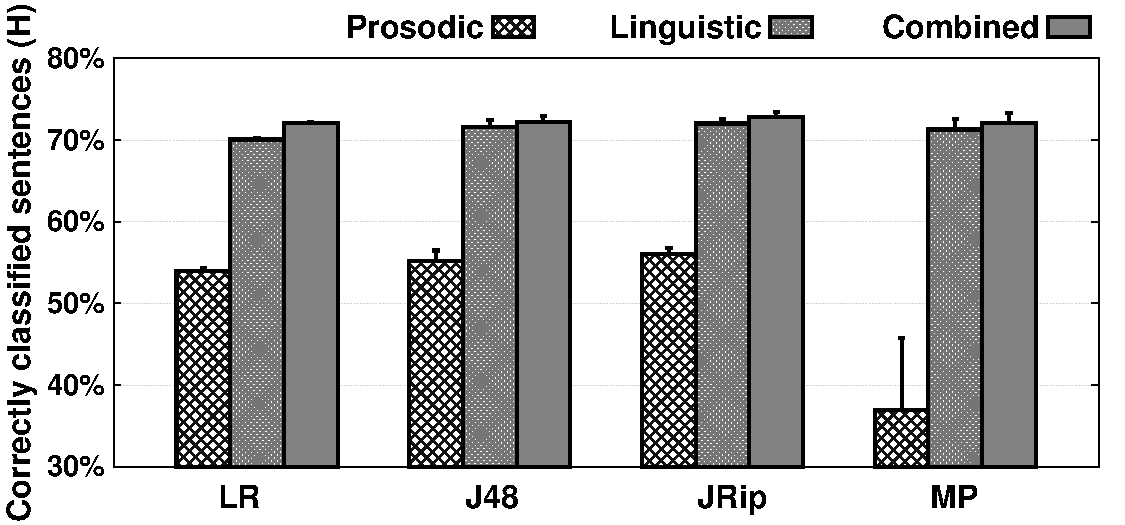
\includegraphics[scale=0.42]{Image/average_PLC_onAutomatic_4colors_withSD_Gray.pdf}}
\hfil
\subfloat[Tests on manual transcriptions]{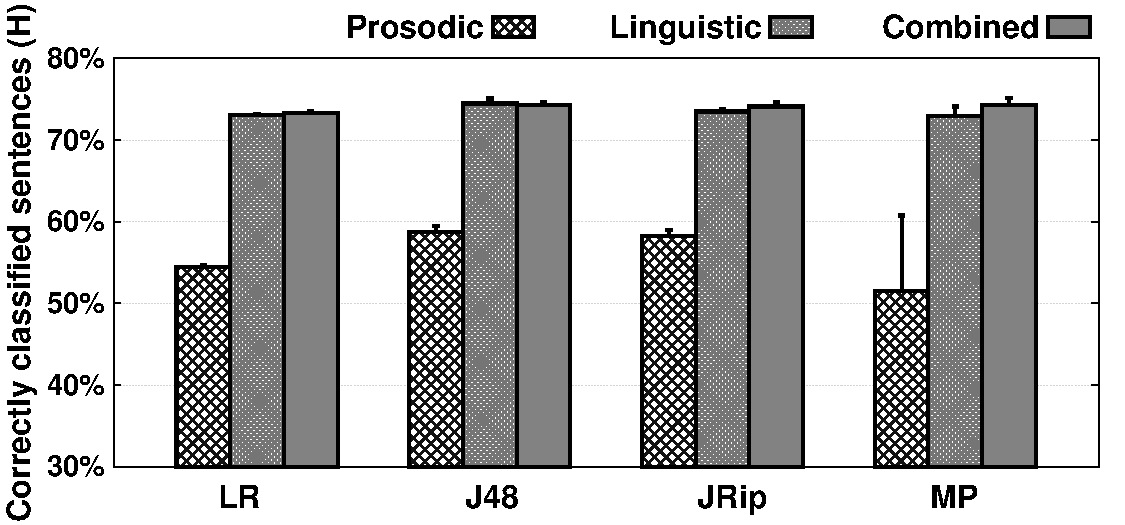
\includegraphics[scale=0.42]{Image/average_PLC_onManual_4colors_withSD_Gray.pdf}}
}
\caption{Analysis of the average classifier's performance when applied on automatic (a) or on manual (b) transcriptions}
\label{Fig:PLC}
\end{figure*}




%=======================================================================================
\section{Experiments and Results}
%=======================================================================================

The classifier evaluations are carried out using features stemming out from: 

\begin{itemize}
\item automatic transcriptions (obtained with a large vocabulary speech recognizer) - to study the performance under real conditions;
\item manual transcriptions - to study the classifier's maximum performance, obtainable only in ideal conditions (i.e. perfect transcript).
\end{itemize}

The performance obtained on our imbalanced test data set (831 questions and 7005 statements) is evaluated by the harmonic mean between the ratio of correctly classified questions and the ratio of correctly classified statements, computed as: 

\noindent
$$\text{H}=\text{2*}\left(\frac{\text{ccQuestions * ccStatements}}{\text{ccQuestions + ccStatements}}\right)$$

\noindent where ``cc" is an acronym for ``correctly classified".
This value allows us to estimate the global performance of our classifier, given that the performance achieved on questions and on statements are equally important.

%%%%%%%%%%%%%%%%%%%%%%%%%%%%%%%%%%%%%%%%%%%%%%%%%%%%%%%%%%%%%%%%%%%%%%%%%%%%%%%%%%%%%%%%%%%%%%%%%%%%%%%%%%%%%%%%%%%%%%%%%%%
\subsection{Results with predefined sentence boundaries}

In this first set of experiments we consider perfect sentence boundaries for the automatic transcriptions (as defined in the manual transcriptions).
 
Figure \ref{Fig:PLC} shows the average performance obtained with all four classifiers on the prosodic, linguistic and combined features, when applied on automatic or on manual transcriptions. 
It can be easily observed that the linguistic classifiers outperform the prosodic classifiers. 
The performance obtained with the linguistic classifiers when applied on the automatic transcriptions and on the manual transcriptions differs by about 3\% absolute, due to recognition errors (22\% word error rate on Ester and 28\% on Etape) and most likely to the misrecognition of the interrogative words.
The combination of linguistic and prosodic features does not provide any improvement on manual transcripts and provides only a slight improvement on automatic transcription.

All four classifiers achieve similar performance when using linguistic or combined features (which are the most useful features). 
Further experiments will be evaluated only with the neural network classifier (MP).


\begin{table}[b!]
\renewcommand{\arraystretch}{1.3}
\caption{Confusion matrix between questions and statements obtained on manual transcriptions}
\label{Tab:cMatrix}
\centering
\begin{tabular}{p{1.01cm}|p{0.7cm}|p{1.3cm}|p{1.3cm}|p{2cm}}
\cline{2-4}
& number & classified as \textbf{Question} & classified as \textbf{Statement} &   \\
\end{tabular}

\begin{tabular}{|p{1cm}|p{0.7cm}|p{1.3cm}|p{1.3cm}|p{2cm}}
\cline{1-4}
\textbf{Question}  &  831 & 603 & 228   & \textbf{ccQuestions=72.56\%} \\ \cline{1-4}
\textbf{Statement} & 7005 & 1559 & 5446  & \textbf{ccStatements=77.74\%} \\ \cline{1-4}
\end{tabular}
\end{table}


More detailed results obtained with the MP classifier on the combined prosodic-linguistic features extracted from manual transcriptions (when trained on a single random training set) are given in table \ref{Tab:cMatrix}.
603 out of 831 questions were correctly classified as questions (ccQuestions=$72.56\%$) and 5446 out of 7005 statements were correctly classified as statements (ccStatements=$77.74\%$). 
The harmonic average performance is here H=$75.05\%$. 

Further analysis on the classification results obtained on automatic transcriptions showed that the data belonging to ESTER2 (prepared speech; average performance of 73\%)  is easier to classify than the data belonging to ETAPE (spontaneous speech; average performance of 70\%).


Figure \ref{Fig:Features} shows the average performance obtained with the MP classifier when using different feature combinations on automatic and manual transcriptions. The most important linguistic feature is the lexical log-likelihood ratio ({\it lexLLR}), with the interrogative patterns ({\it iP}) and the syntactic log-likelihood ratio ({\it synLLR}) providing complementary information in combination ({\it Linguistic}). 
 
\begin{figure}[b!] 
\centering
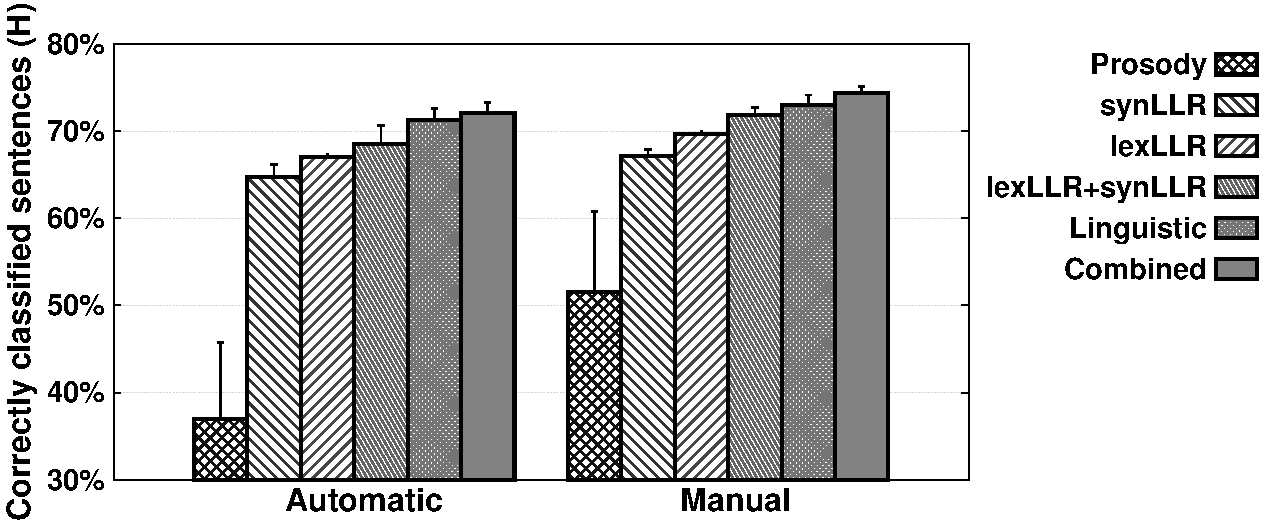
\includegraphics[scale=0.39]{Image/MP_averageStats_compareFeatures_withSD_Gray.pdf}
\caption{Analysis of the average performance obtained with the MP classifier when using different feature combinations on automatic and manual transcriptions}
\label{Fig:Features}
\end{figure}




\begin{figure}[t!] 
\begin{center}
	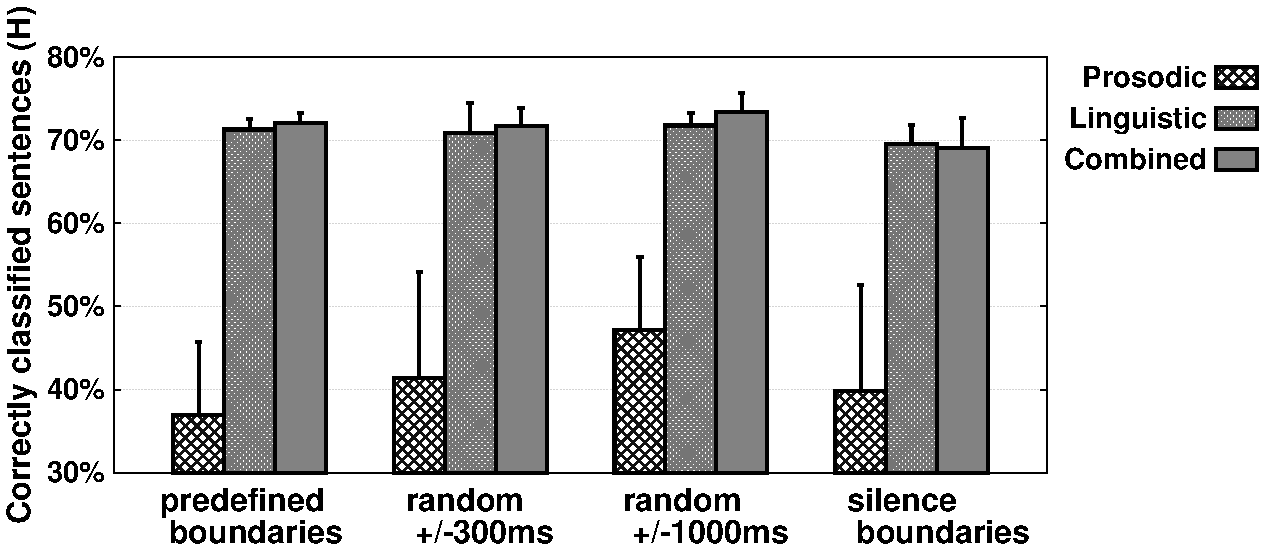
\includegraphics[scale=0.395]{Image/MP_averageStats_differentBorders_Gray.pdf}
	\caption{Analysis of the average performance obtained with the MP classifier on automatic transcriptions when modifying the predefined boundaries}
\label{Fig:Borders}
\end{center}
\end{figure}

%%%%%%%%%%%%%%%%%%%%%%%%%%%%%%%%%%%%%%%%%%%%%%%%%%%%%%%%%%%%%%%%%%%%%%%%%%%%%%%%%%%%%%%%%%%%%%%%%%%%%%%%%%%%%%%%%%%%%%%%%%%
\subsection{Impact of sentence boundary derivations}

Here we want to assess the performance loss when the sentence boundaries are not perfect. To evaluate that, the predefined sentence boundaries are modified to simulate errors introduced by an automatic sentence segmentation. 
We thus modified the sentence boundaries in three different ways : 
\begin{itemize}
\item by shifting each boundary (left and right) with a random value of \{-300, -200, -100, +100, +200, +300\} ms
\item by shifting each boundary (left and right) with a random value of \{-1000, -800, -600, -400, -200, +200, +400, +600, +800, +1000\} ms
\item by finding the longest silence-enclosed sentence : if the sentence has a preceding and a succeeding silence, keep it as it is; else, replace the left boundary with the end of the first succeeding silence and the right boundary with the start of the first preceding silence.
\end{itemize} 


Figure \ref{Fig:Borders} shows the MP's performance loss when changing the predefined sentence boundaries of the automatic transcriptions. 
When we change the sentence boundaries with random values ({\it randomBoundaries:+/-300ms, randomBoundaries:+/-1000ms}), the performance loss of the combined classifier is minimal. 
This can be explained by the fact that we only add or delete few words (at the beginning or end of the sentence).
But when we change the boundaries to their longest silence-enclosed sentence - {\it silenceBoundaries}, the performance loss is bigger. 
But even so, the biggest performance loss amounts to only 3\%.


%%%%%%%%%%%%%%%%%%%%%%%%%%%%%%%%%%%%%%%%%%%%%%%%%%%%%%%%%%%%%%%%%%%%%%%%%%%%%%%%%%%%%%%%%%%%%%%%%%%%%%%%%%%%%%%%%%%%%%%%%%%
\section{Conclusions}

This paper analyzed the detection of sentence modality (questions versus statements) in French when applied on automatic speech-to-text transcriptions. The context of this work is to support the communication with deaf or hard of hearing people, which requires an automatic detection of questions in order to inform them that a question was directed to them. The experiments were carried out using three French speech corpora: ETAPE, EPAC and ESTER2. 

The prosodic classifier gives poor classification results. 
The linguistic classifier provides by far better results: 72\% when it is applied on ASR transcripts (with perfect sentence boundaries) versus 74\% when it is applied on reference manual transcripts. The combination of prosodic and linguistic features provides a slight improvement when applied on automatic transcriptions.

The most useful feature is provided by the word n-grams. However, the performance is highly enhanced with the complementary information provided by the 'discriminative interrogative patterns' feature and by the POS-based n-grams. 

A complementary study was conducted on the automatic transcriptions in order to determine the performance loss when the sentence boundaries are not perfect. 
This was evaluated by modifying the predefined boundaries.
The biggest performance loss amounts to only 3\%. 
This means that even if an automatic segmentation module wrongly assigns the sentence boundaries, our classifier still manages to correctly classify the question-statements entries between 69\% and 72\%.     
  
Future work will investigate further prosodic and linguistic features; confidence measures will also be considered in the computation of the linguistic features.


%%%%%%%%%%%%%%%%%%%%%%%%%%%%%%%%%%%%%%%%%%%%%%%%%%%%%%%%%%%%%%%%%%%%%%%%%%%%%%%%%%%%%%%%%%%%%%%%%%%%%%%%%%%%%%%%%%%%%%%%%%%
\section*{Acknowledgements}

The work presented in this article is part of the RAPSODIE project, and has received
support from the ``Conseil R\'{e}gional de Lorraine" and from the ``R\'{e}gion Lorraine" (FEDER) (http://erocca.com/rapsodie).


%=======================================================================================
% references section
%=======================================================================================

% trigger a \newpage just before the given reference number - balance the columns on the last page; adjust value as needed - readjust if the document is modified later

%\IEEEtriggeratref{8}

% The "triggered" command can be changed if desired:
%\IEEEtriggercmd{\enlargethispage{-5in}}

\bibliographystyle{IEEEtran}
\bibliography{myBib_QD}

\end{document}


